En esta sección detallaremos cada unos de los datasets usados durante nuestro trabajo, las distintas fuentes de atributos, y el esquema de clasificación usado.

\section{Análisis de los Datasets}

\subsection{Dataset VarQ}

El primer paso que tomamos fue realizar un análisis del dataset VarQ. Este dataset fue generado por la herramienta homónima generada en el BIA (Plataforma Bioinformática Argentina) por Leandro Radusky. Esta herramienta permite extraer datos estructurales de variantes proteicas de un sólo aminoácido (SAS, por sus siglas en inglés) tomando información de diferentes bases de datos o aplicaciones (PDB, PFam, 3DID, entre otras), permitiendo el análisis manual de los diferentes cambios estructurales, como el tipo de actividad, el plegamiento, si pertenece a un sitio activo, o si forma parte en interfaces proteína-proteína \cite{Radusky2017}. 

\begin{figure}[H]
    \centering
    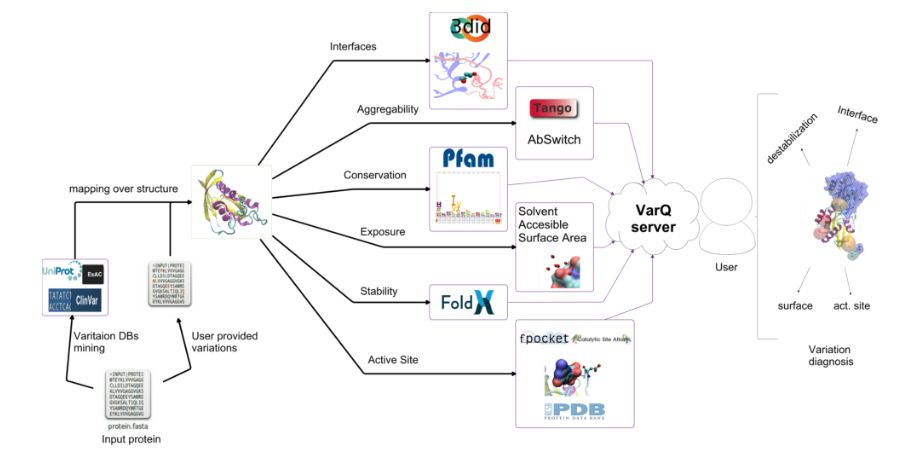
\includegraphics[scale=0.4]{documents/latex/figures/1/pipeline.png}
    \caption{Pipeline de extracción de datos de la herramienta VarQ. Esta figura fue extraída de la tesis de doctorado de Leandro Radusky.}
    \label{fig:varq_pipeline}
\end{figure}


Este dataset fue un acercamiento inicial al problema de predecir si a partir de una mutación en el gen. Para esto verificamos la calidad de cada una de las variables incluyendo el tipo. Validando el tipo de cada una de las variantes pudimos encontrar algunas de las que no se conoce a ciencia cierta su patogenicidad, por lo que fueron removidas. El dataset VarQ final tiene aproximadamente 17,8 mil variantes, de los cuales:

\begin{itemize}
    \item 11,7 mil están catalogados como benignos.
    \item 6,1 mil están catalogados como patogénicos.
\end{itemize}

Posee 12 columnas o variables: 

\begin{itemize}
    \item Mutant: Código identificatorio de la variante, compuesto por el código Uniprot, la posición del aminoácido donde ocurre la variación, y el cambio de aminoácido.
    \item SASA (Solvent-Accessible Surface Area): El área del aminoácido accesible por un solvente.
    \item SASA Percentage: El porcentaje del SASA sobre la superficie del aminoácido.
    \item B-FACTOR: Factor de temperatura correspondiente a un aminoácido en la proteína. Una mayor temperatura indica que el aminoácido pertenece a una zona potencialmente de mayor movilidad.
    \item Switchability: Factor de \textit{switching} del aminoácido \cite{Diaz2014}. Genera cambios en el plegamiento y por ende en la función de la proteína. 
    \item Aggregability: Usando el software Tango \cite{Fernandez-Escamilla2004}, evalúa la propensión del aminoácido a generar agregación desde un punto de vista estructural
    
\end{itemize}

\subsection{Humsavar}

Humsavar es una recopilación de SNPs anotados manualmente 


\section{Variables}

\subsection{ProtParam}

\subsection{VEST}

\subsection{SNVBox}


\section{Esquema de Clasificación}